\documentclass[a4paper]{article}
\usepackage{amsmath}
\usepackage{geometry}
\usepackage{float}
\geometry{a4paper, left=2.54cm, right=2.54cm, top=2.54cm, bottom=2.54cm}
\usepackage{indentfirst}
\usepackage{enumitem}
\usepackage{bm}
% 段落間距  (begin doc 才設定)
\usepackage{parskip}
    % 普通文字,行距
    \usepackage[onehalfspacing]{setspace}
    
\usepackage{tabularx}

\usepackage{fontspec,xltxtra,xunicode}


\setmainfont{Times New Roman}
\usepackage{xeCJK}
\setCJKmainfont[AutoFakeBold=3]{DFKai-SB} %设置中文字体\XeTeXlinebreaklocale “zh”\XeTeXlinebreakskip = 0pt plus 1pt minus 0.1pt %文章内中文自动换行


\usepackage{minted}
\renewcommand{\theFancyVerbLine}{\sffamily\small\arabic{FancyVerbLine}}
\setminted{
  baselinestretch=1,
  fontsize=\fontsize{10pt}{12pt},
  python3=true,
  style=tango,
  linenos=true,
  xleftmargin=20pt,     % 控制行号距离左侧的距离
  frame = single
}




\usepackage{caption}
\newenvironment{code}{\captionsetup{type=listing, font=large, name=List.}}{}
\captionsetup{font={large}}


\usepackage{titlesec}



\def\Large{\fontsize{18}{20}\selectfont}
\def\huge{\fontsize{26}{10}\selectfont}
\def\Huge{\fontsize{36}{54}\selectfont}

\titleformat{\section}
  {\fontsize{18pt}{15}\bfseries}
  {\selectfont\thesection.}
  {0.5em}
  {}

  \titleformat{\subsection}
  {\fontsize{16pt}{15}\bfseries}
  {\selectfont\thesubsection.}
  {0.5em}
  {}

\usepackage{longtable}
\usepackage{array}
\renewcommand{\arraystretch}{1.2}

\renewcommand{\figurename}{Fig.}


\title{\textbf{{\huge Code - HW2} \\ 記憶體積體電路\ Memory\ Circuit\ Design}}
\author{{\Large\textbf{ 電機4A\quad 109501201\quad 陳緯亭}}}
\date{\Large{\today}} 

\begin{document}

\newcolumntype{L}[1]{>{\raggedright\let\newline\\\arraybackslash\hspace{0pt}}m{#1}}
\newcolumntype{C}[1]{>{\centering\let\newline\\\arraybackslash\hspace{0pt}}m{#1}}
\newcolumntype{R}[1]{>{\raggedleft\let\newline\\\arraybackslash\hspace{0pt}}m{#1}}


\maketitle

\fontsize{14pt}{1em}

\selectfont

\section{DC Analysis}

\subsection{6T SRAM}

做 Decouple,畫雙曲線。\\要RSNM圖,X-Y軸分別為 VIN-Q1,和 Q1-VIN。\\
要 WNM圖,X-Y軸分別為VIN-Q1,和 Q2-VIN。

\begin{figure}[!htbp]
\centering
\begin{minipage}[t]{0.45\textwidth}
\centering
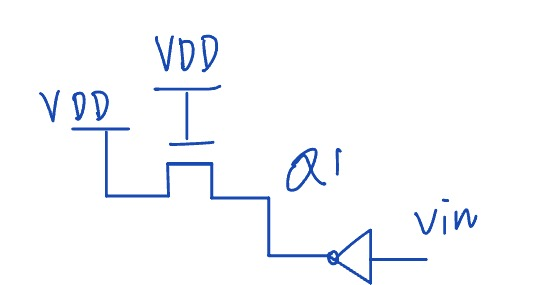
\includegraphics[width=\linewidth]{./img/2023-11-16-14-50-00.png}
\caption{Decouple (to VDD)}
\label{r}
\end{minipage}
\qquad
\begin{minipage}[t]{0.4\textwidth}
\centering
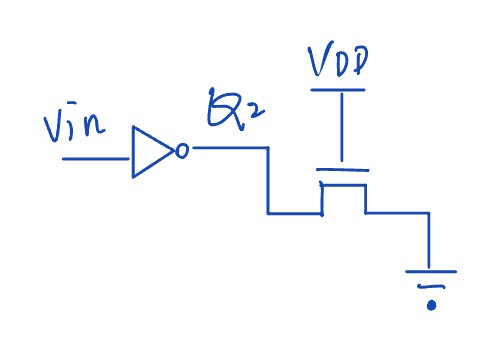
\includegraphics[width=\linewidth]{./img/2023-11-16-14-52-25.png}
\caption{Decouple (to GND)}
\label{w}
\end{minipage}
\end{figure}


\begin{code}
\caption{DC Analysis - 6T SRAM}
\label{inv}
\begin{minted}[linenos, breaklines]{spice}
*** SRAM 6T curve ***
*** .protect
.inc "/home/college/c109501201/Memory/65nm_bulk.pm"
.unprotect
*** 
.param V1 = 1
.param V08 = 0.8
.param V06 = 0.6
.param V04 = 0.4
***
.global VDD1! VSS! VDD08! VDD06! VDD04!
VDD1   VDD1! 0    dc V1
VDD08  VDD08! 0   dc V08
VDD06  VDD06! 0   dc V06
VDD04  VDD04! 0   dc V04
VSS    VSS! 0    dc  0

***inverter
** Mos D G S B
** .ic 是初始偏壓值
.subckt inv in out Wp = 1 Wn = 1 VDD = V1
.ic VDD! = VDD 
Mp out in VDD! VDD! pmos w= 'Wp * 1u' l=65n m=1
Mn out in VSS! VSS! nmos w= 'Wn * 1u' l=65n m=1
.ends

*** source
va vin gnd


*** Vdd = 1V read write
xinv1 vin 1 inv VDD = V1 Wp = 0.25 Wn = 0.2
Mn1 VDD1!  VDD1! 1 gnd nmos w = 0.2u l = 0.065u 

*** Vdd = 1V write 
xinv5 vin 5 inv VDD = V1 Wp = 0.25 Wn = 0.2
Mn5 5  VDD1! gnd gnd nmos w = 0.2u l = 0.065u

*** Vdd = 0.8V read write
xinv2 vin 2 inv VDD = V08 Wp = 0.25 Wn = 0.2
Mn2 VDD08! VDD08! 2 gnd nmos w = 0.2u l = 0.065u

*** Vdd = 0.8V write
xinv6 vin 6 inv VDD = V08 Wp = 0.25 Wn = 0.2
Mn6 6  VDD08! gnd gnd nmos w = 0.2u l = 0.065u

*** Vdd = 0.6V read write
xinv3 vin 3 inv VDD = V06 Wp = 0.25 Wn = 0.2
Mn3 VDD06! VDD06! 3 gnd nmos  w = 0.2u l = 0.065u

*** Vdd = 0.6V write
xinv7 vin 7 inv VDD = V06 Wp = 0.25 Wn = 0.2
Mn7 7  VDD06! gnd gnd nmos w = 0.2u l = 0.065u

*** Vdd = 0.4V read write
xinv4 vin 4 inv VDD = V04 Wp = 0.15 Wn = 0.1
Mn4 VDD04! VDD04! 4 gnd nmos w= 0.3u l = 0.1u

*** Vdd = 0.4V write write
xinv8 vin 8 inv VDD = V04 Wp = 0.15 Wn = 0.1
Mn8 8  VDD04! gnd gnd nmos w = 0.3u l = 0.1u

*** only the first dc is effective
.dc va 0 V06 0.02V
.dc va 0 V08 0.02V
.dc va 0 V1 0.02V
.dc va 0 V04 0.01V
.option post
.end
\end{minted}
\end{code}

\subsection{8T SRAM}

做 Decouple,畫雙曲線。\\要RSNM圖,X-Y軸分別為 Q-QB,和 QB-Q。\\
要 WNM圖,X-Y軸分別為Q-QB,和 QB1-Q。

\begin{figure}[!htbp]
\centering
\begin{minipage}[t]{0.45\textwidth}
\centering
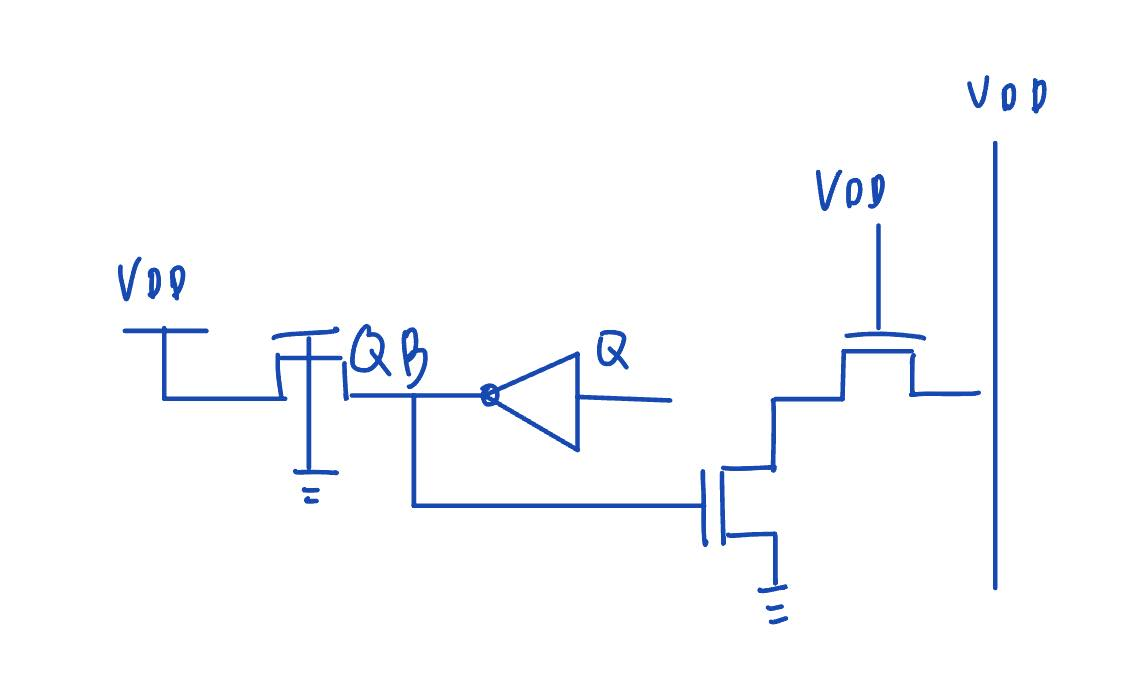
\includegraphics[width=\linewidth]{./img/2023-11-16-15-44-00.png}
\caption{Decouple (to VDD)}
\label{r8}
\end{minipage}
\qquad
\begin{minipage}[t]{0.4\textwidth}
\centering
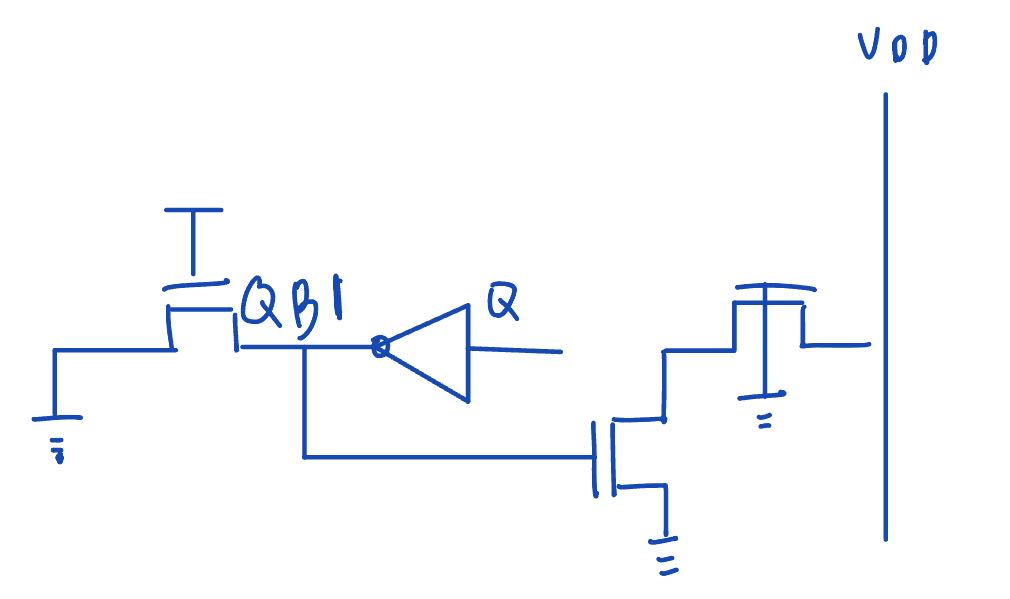
\includegraphics[width=\linewidth]{./img/2023-11-16-15-45-01.png}
\caption{Decouple (to GND)}
\label{w8}
\end{minipage}
\end{figure}



\begin{code}
\caption{DC Analysis - 8T SRAM}
\begin{minted}[linenos, breaklines]{spice}
* 8T SRAM Cell - HSPICE Netlist
* .protect
.include "/home/college/c109501201/Memory/65nm_bulk.pm"
.unprotect

* Parameters
.param V1 = 1
.param V08 = 0.8
.param V06 = 0.6
.param V04 = 0.4

*** 改這裡
.param VDD = 'V04'


* Global Nodes
.global VDD! VSS!
* Power Supplies
VDD   VDD! 0 dc VDD
VSS    VSS! 0 dc 0

* Inverter Subcircuit
.subckt inv in out Wp=1 Wn=1 VDD=VDD
.IC VDD = VDD
Mpos out in VDD VDD PMOS L=65n W='Wp*1u' AD=1 PD=1
Mneg out in VSS! VSS! NMOS L=65n W='Wn*1u' AD=1 PD=1
.ends

* Source
VBLB BLB GND dc VDD
** 注意 WL = 0V
Vw WL GND dc 0 
VRDWL RDWL 0 dc VDD
VRDBL RDBL 0 dc VDD
VQ Q 0 dc 0
Vwl1 WL1 GND dc VDD
VBL0 BL0 GND dc 0
VRDW0 RDW0 GND dc 0
.param p1 = 0.7
.param n1 = 0.4
.param w1 = 0.6u
.param l1 = 0.065u
* Read Operation
MN8 RDBL RDWL X GND NMOS W=w1 L=l1
MN9 X QB GND GND NMOS W=w1 L=l1
xinv2 Q QB  inv VDD=VDD Wp=p1 Wn= n1
MN5 BLB WL QB GND NMOS W=w1 L=l1

* Write Operation
MN81 RDBL RDW0 X1 GND NMOS W=w1 L=l1
MN91 X1 QB1 GND GND NMOS W=w1 L=l1
xinv4 Q QB1  inv VDD=VDD Wp=p1 Wn= n1
MN51 BL0 WL1 QB1 GND NMOS W=w1 L=l1

* DC Analysis
.dc VQ 0 VDD 0.01V

.option post
.end
\end{minted}
\end{code}

\section{Transient Analysis}


\subsection{6T SRAM}

\begin{figure}[H]
\centering
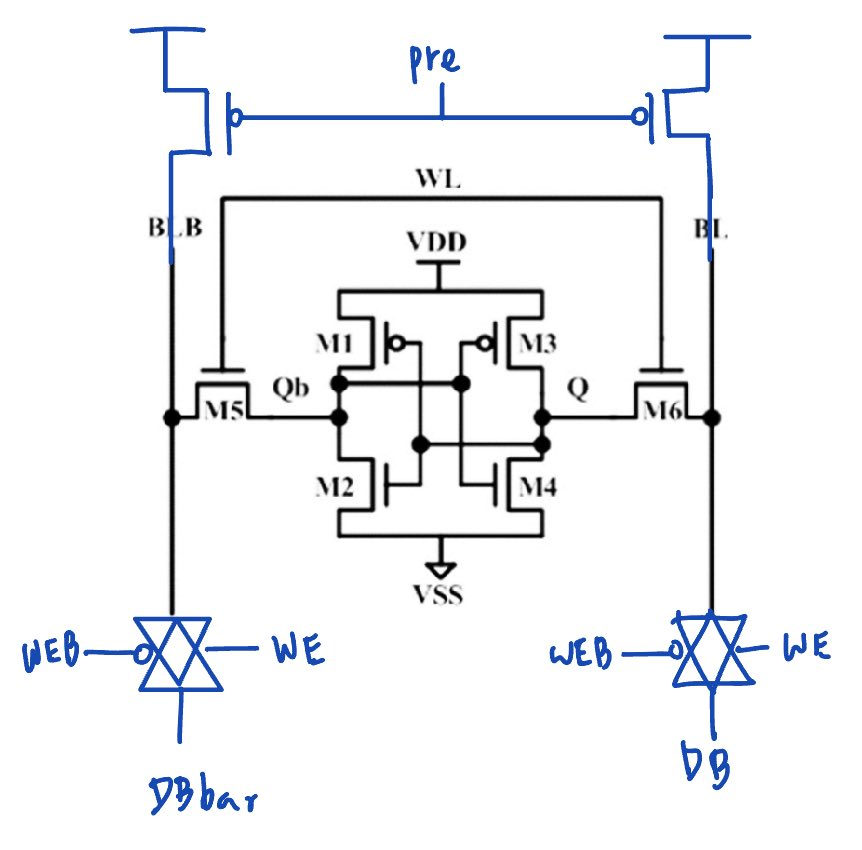
\includegraphics[width=0.7\textwidth]{./img/2023-11-16-15-55-26.png}
\caption{Transient Analysis - 6T SRAM}
\end{figure}

\begin{code}
\caption{Transient Analysis - 6T SRAM}
\begin{minted}[linenos, breaklines]{spice}
*** SRAM6T Transient Analysis ***
*** .protect
.inc "/home/college/c109501201/Memory/65nm_bulk.pm"
.unprotect
*** 

.param VDD = 0.8
***
.global VSS! VDD!
VDD  VDD! 0   dc VDD
VSS    VSS! 0    dc  0

***inverter
** Mos D G S B
** .ic 是初始偏壓值
.subckt inv in out Wp = 1 Wn = 1
Mp out in VDD! VDD! pmos w= 'Wp * 1u' l=65n m=1
Mn out in VSS! VSS! nmos w= 'Wn * 1u' l=65n m=1
.ends

VWL   WL VSS! pulse(VDD 0V 0ns 0.05ns 0.05ns 2ns 4ns)
VPRE PRE VSS! pulse(0V VDD -1ns 0.05ns 0.05ns 5ns 8ns)
VWE   WE VSS! pulse(0V VDD 0ns 0.05ns 0.05ns 4ns 8ns)
VD    D VSS! pulse(VDD 0 0ns 0.05ns 0.05ns 8ns 16ns)
VDB DBbar VSS! pulse(0 VDD 0ns 0.05ns 0.05ns 8ns 16ns)
xweb WE WEB inv Wp = 0.25 Wn = 0.2

Mpl BL PRE  VDD! VDD! pmos w = 0.1u l = 65n
Mp2 BLB PRE VDD! VDD! pmos w = 0.1u l = 65n

Mn1 D     WE BL  gnd nmos w = 0.1u l =65n
Mp3 D     WEB BL  gnd pmos w = 0.1u l =65n
Mn2 DBbar WE BLB gnd  nmos w =  0.1u l =65n
Mp4 DBbar WEB BLB gnd pmos w = 0.1u l =65n
*** read source
* Vpre pre VSS! pulse(0V 0.8V 0.5ns 0.05ns 0.05ns 2ns 4ns)

*** 要改
* .IC V(Q) = VDD
* VBL preBL VSS! pulse(0.8V 0V 0ns 0.05ns 0.05ns 4ns 16ns)
* VBLB preBLB VSS! pulse(0V 0.8V 0ns 0.05ns 0.05ns 8ns 12ns)
* .IC V(BL)=VDD
* .IC V(BLB)=VDD

*** Write Source
* .IC V(Q) = 0
* vblin BL VSS! pulse(0V 0.8V 0ns 0.5ns 0.5ns 1ns 4ns)
* vblbin BLB VSS! pulse(0.8V 0V 0ns 0.5ns 0.5ns 1ns 4ns)

xinv1 QB Q inv Wp = 0.25 Wn = 0.2
Mn6 Q WL BL  gnd nmos w = 0.3u l = 0.2u

xinv2 Q QB inv Wp = 0.25 Wn = 0.2
Mn5  QB WL BLB gnd nmos w = 0.3u l = 0.2u

*** Power Analysis
.probe PWR_BLB =  'I(Mn5)'*'V(BLB)'
.probe PWR_BL =  'I(Mn6)'*'V(BL)'
.tran    1p    17ns 
.MEAS TRAN AvgPower AVG(power) FROM=1pS TO=10ns

.option post
.end  
\end{minted}
\end{code}

\subsection{8T SRAM}

\begin{figure}[H]
  \centering
  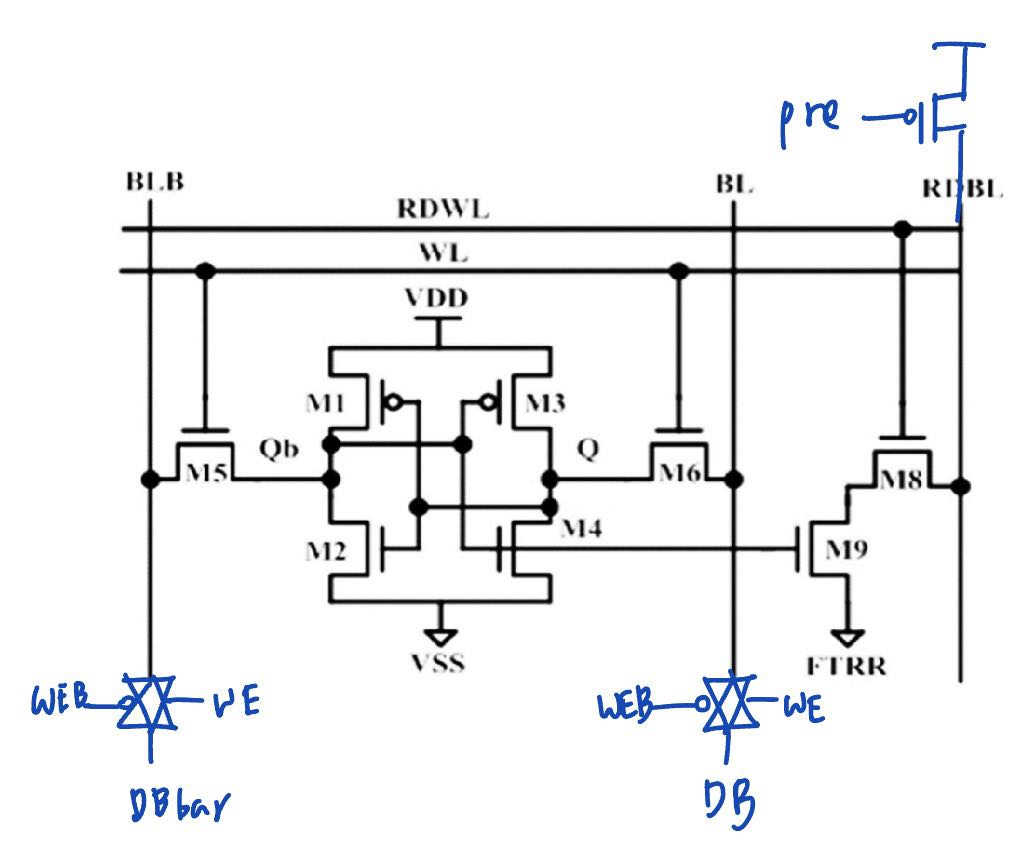
\includegraphics[width=0.7\textwidth]{./img/2023-11-16-16-28-53.png}
  \caption{Transient Analysis - 8T SRAM}
  \end{figure}

\begin{code}
\caption{Transient Analysis - 8T SRAM}
\begin{minted}[linenos, breaklines]{spice}
*** SRAM8T Transient Analysis ***
*** .protect
.inc "/home/college/c109501201/Memory/65nm_bulk.pm"
.unprotect
*** 

.param VDD = 0.8
***
.global VSS! VDD!
VDD  VDD! 0   dc VDD
VSS    VSS! 0    dc  0

***inverter
** Mos D G S B
** .ic 是初始偏壓值
.subckt inv in out Wp = 1 Wn = 1
Mp out in VDD! VDD! pmos w= 'Wp * 1u' l=65n m=1
Mn out in VSS! VSS! nmos w= 'Wn * 1u' l=65n m=1
.ends


VWL   WL VSS! pulse(VDD 0V 0ns 0.05ns 0.05ns 2ns 4ns)
VPRE PRE VSS! pulse(0V VDD -1ns 0.05ns 0.05ns 5ns 8ns)
VWE   WE VSS! pulse(0V VDD 0ns 0.05ns 0.05ns 4ns 8ns)
VD    D VSS! pulse(VDD 0 0ns 0.05ns 0.05ns 8ns 16ns)
VDB DBbar VSS! pulse(0 VDD 0ns 0.05ns 0.05ns 8ns 16ns)
VRDWL RDWL VSS! dc VDD
xweb WE WEB inv Wp = 0.25 Wn = 0.2

Mpl RDBL PRE  VDD! VDD! pmos w = 0.1u l = 65n

Mn1 D     WE BL  gnd nmos w = 0.1u l =65n
Mp3 D     WEB BL  gnd pmos w = 0.1u l =65n
Mn2 DBbar WE BLB gnd  nmos w =  0.1u l =65n
Mp4 DBbar WEB BLB gnd pmos w = 0.1u l =65n

*** Read source
* VRDWL RDWL  VSS! pulse(0V 0.8V 0.5ns 0.1ns 0.1ns 1ns 2ns)
* VWL WL VSS! dc 0
* .IC V(Q)=VDD
* .IC V(RDBL)=VDD
* VPRE PRE VSS! pulse(0V 0.8V 0.5ns 0.5ns 0.5ns 1ns 2ns)

* .IC V(BL)=VDD
* .IC V(BLB)=VDD

*** Write source
* .IC V(Q) = 0
* VWL WL  VSS! pulse(0V 0.8V 0.5ns 0.05ns 0.05ns 1ns 2ns)
* vblin BL VSS! pulse(0V 0.8V 0ns 0.5ns 0.5ns 1ns 4ns)
* vblbin BLB VSS! pulse(0.8V 0V 0ns 0.5ns 0.5ns 1ns 4ns)

* MPpre RDBL PRE VDD! VDD!  pmos W=0.5u L=65n

xin1 QB Q inv Wp=0.13 Wn=0.13
MN8 RDBL RDWL X GND NMOS W=0.5u L=65n
MN9 X QB GND GND NMOS W=0.5u L=65n
MN6 BL WL Q GND NMOS W=0.3u L=0.16u
xinv2 Q QB  inv Wp=0.13 Wn=0.13
MN5 BLB WL QB GND NMOS W=0.3u L=0.16u

*** Power Analysis
.probe PWR_BLB =  'I(MN5)'*'V(BLB)'
.probe PWR_BL =  'I(MN6)'*'V(BL)'

.tran    1p    16ns 
.MEAS TRAN AvgPower AVG(power) FROM=1pS TO=10ns
.option post
.end  
\end{minted}
\end{code}

\section{Power Analysis}

2、3 題 Code 同一份。

\section*{Matlab Code for Question 1}

\begin{code}
\caption{Matlab code for Q1}
\begin{minted}[linenos, breaklines]{matlab}
% Specify the Excel file path
excelFilePath = "D:\Document\Senior\Memory_Circuit_Design\HW2\SRAM8T.xlsx";
% Read data from Excel
data = xlsread(excelFilePath, 4);

close; 
% Extract data
VI = data(:, 1);  % Assuming VI is in the first column
VOr = data(:, 2);
VOw = data(:, 3);
%VOgnd = data(:, 2);  % Assuming VO is in the second column
%VOVdd = data(:, 3);

% Plot SNM
figure(1);
width=500;%宽度,像素数
height=500;%高度
left=200;%距屏幕左下角水平距离
bottem=200;%距屏幕左下角垂直距离
set(gcf,'position',[left,bottem,width,height])
plot(VI, VOr, 'b-', 'LineWidth', 2);
hold on;
plot(VOr, VI, 'g-', 'LineWidth', 2);
hold on;

figure(2);
width=500;%宽度,像素数
height=500;%高度
left=200;%距屏幕左下角水平距离
bottem=200;%距屏幕左下角垂直距离
set(gcf,'position',[left,bottem,width,height])
plot(VI, VOr, 'b-', 'LineWidth', 2);
hold on;
plot(VOw, VI, 'g-', 'LineWidth', 2);
hold on;
\end{minted}
\end{code}

\end{document}